\section{Problem Description}
\begin{frame}
	\frametitle{$k$-connected graphs}
	\begin{itemize}
		\item Connectivity
			\begin{itemize}
				\item The minimum number of vertices which need to be removed to disconnect the graph 
			\end{itemize}
		\item $G$ is $k$-connected if it's connectivity is $k$
	\end{itemize}
	\begin{figure}
		\begin{center}
			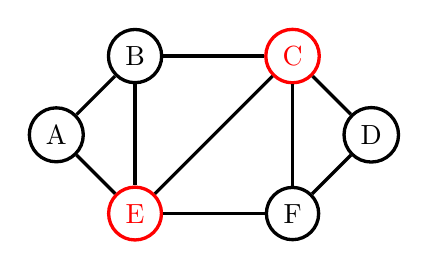
\begin{tikzpicture}[scale=0.5]
  \node[draw,circle, very thick] (A) at (0,2) {A};
  \node[draw,circle, very thick] (B) at (2,4) {B};
  \node[draw,circle, very thick, color=red] (C) at (6,4) {C};
  \node[draw,circle, very thick] (D) at (8,2) {D};
  \node[draw,circle, very thick, color=red] (E) at (2,0) {E};
  \node[draw,circle, very thick] (F) at (6,0) {F};
  \draw[very thick] (A) -- (B);
  \draw[very thick] (A) -- (E);
  \draw[very thick] (B) -- (C);
  \draw[very thick] (B) -- (E);
  \draw[very thick] (C) -- (D);
  \draw[very thick] (C) -- (E);
  \draw[very thick] (C) -- (F);
  \draw[very thick] (D) -- (F);
  \draw[very thick] (E) -- (F);
\end{tikzpicture}

		\end{center}
		\caption{A 2-connected graph}
	\end{figure}
\end{frame}

%TODO less maths
\begin{frame}
  \frametitle{$k$-partition}
  \begin{itemize}
  \item Obtain $\{V_1, \dots, V_k\}$ with
    \begin{itemize}
    \item $\forall i, \lceil V_i \rceil$ is connected
    \item $\sum\limits_{i=0}^k|V_i| = |V|$
    \item $\forall i,j \in \{1, \dots, k\}^2, i \neq j, V_i \cap V_j = \emptyset$
    \end{itemize}
  \end{itemize}
  \begin{figure}
    \begin{center}
      
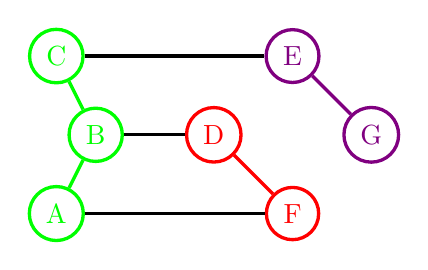
\begin{tikzpicture}[scale=0.5]
  \node[draw,circle, very thick, color=green] (A) at (0,0) {A};
  \node[draw,circle, very thick, color=green] (B) at (1,2) {B};
  \node[draw,circle, very thick, color=green] (C) at (0,4) {C};
  \node[draw,circle, very thick, color=red] (D) at (4,2) {D};
  \node[draw,circle, very thick, color=violet] (E) at (6,4) {E};
  \node[draw,circle, very thick, color=red] (F) at (6,0) {F};
  \node[draw,circle, very thick, color=violet] (G) at (8,2) {G};
  \draw[color=green, very thick] (A) -- (B);
  \draw[color=green, very thick] (B) -- (C);
  \draw[very thick] (B) -- (D);
  \draw[very thick] (A) -- (F);
  \draw[very thick] (C) -- (E);
  \draw[very thick, color=violet] (E) -- (G);
  \draw[very thick, color=red] (D) -- (F);
\end{tikzpicture}

    \end{center}
    \caption{A 3-partition graph}
  \end{figure}
\end{frame}

\begin{frame}
  \frametitle{Article Description}
  \begin{itemize}
  \item Finding a $k$-partition
    \begin{itemize}
    \item In a $k$-connected graph
    \item Choosing $k$ vertices $\{a_1, \dots , a_k\}$
    \item Choosing the size of each component $\{n_1, \dots ,n_k\}$,
      $\sum\limits_{i}^k{n_i} = n$
    \item Complexity : $O(k^2 n^2)$
    \end{itemize}
%    \begin{itemize}
%    \item National audience
%    \item Bimonthly published
%    \end{itemize}
  \end{itemize}
\end{frame}


